\documentclass{standalone}
%\usepackage{auto-pst-pdf,pst-barcode}
\usepackage{pstricks-add}
\usepackage{tikz}
\usepackage{tikz-3dplot}
\usetikzlibrary{3d}
\usepackage{parskip}
\usepackage{tkz-berge}
\usetikzlibrary{shapes.geometric}
\usetikzlibrary{shapes}

\tikzset{My Arrow Style/.style={single arrow, fill=red!50, anchor=base, align=center,text width=15.8cm}}
\newcommand{\MyArrow}[2][]{\tikz[baseline] \node [My Arrow Style,#1] {#2};}

\begin{document}

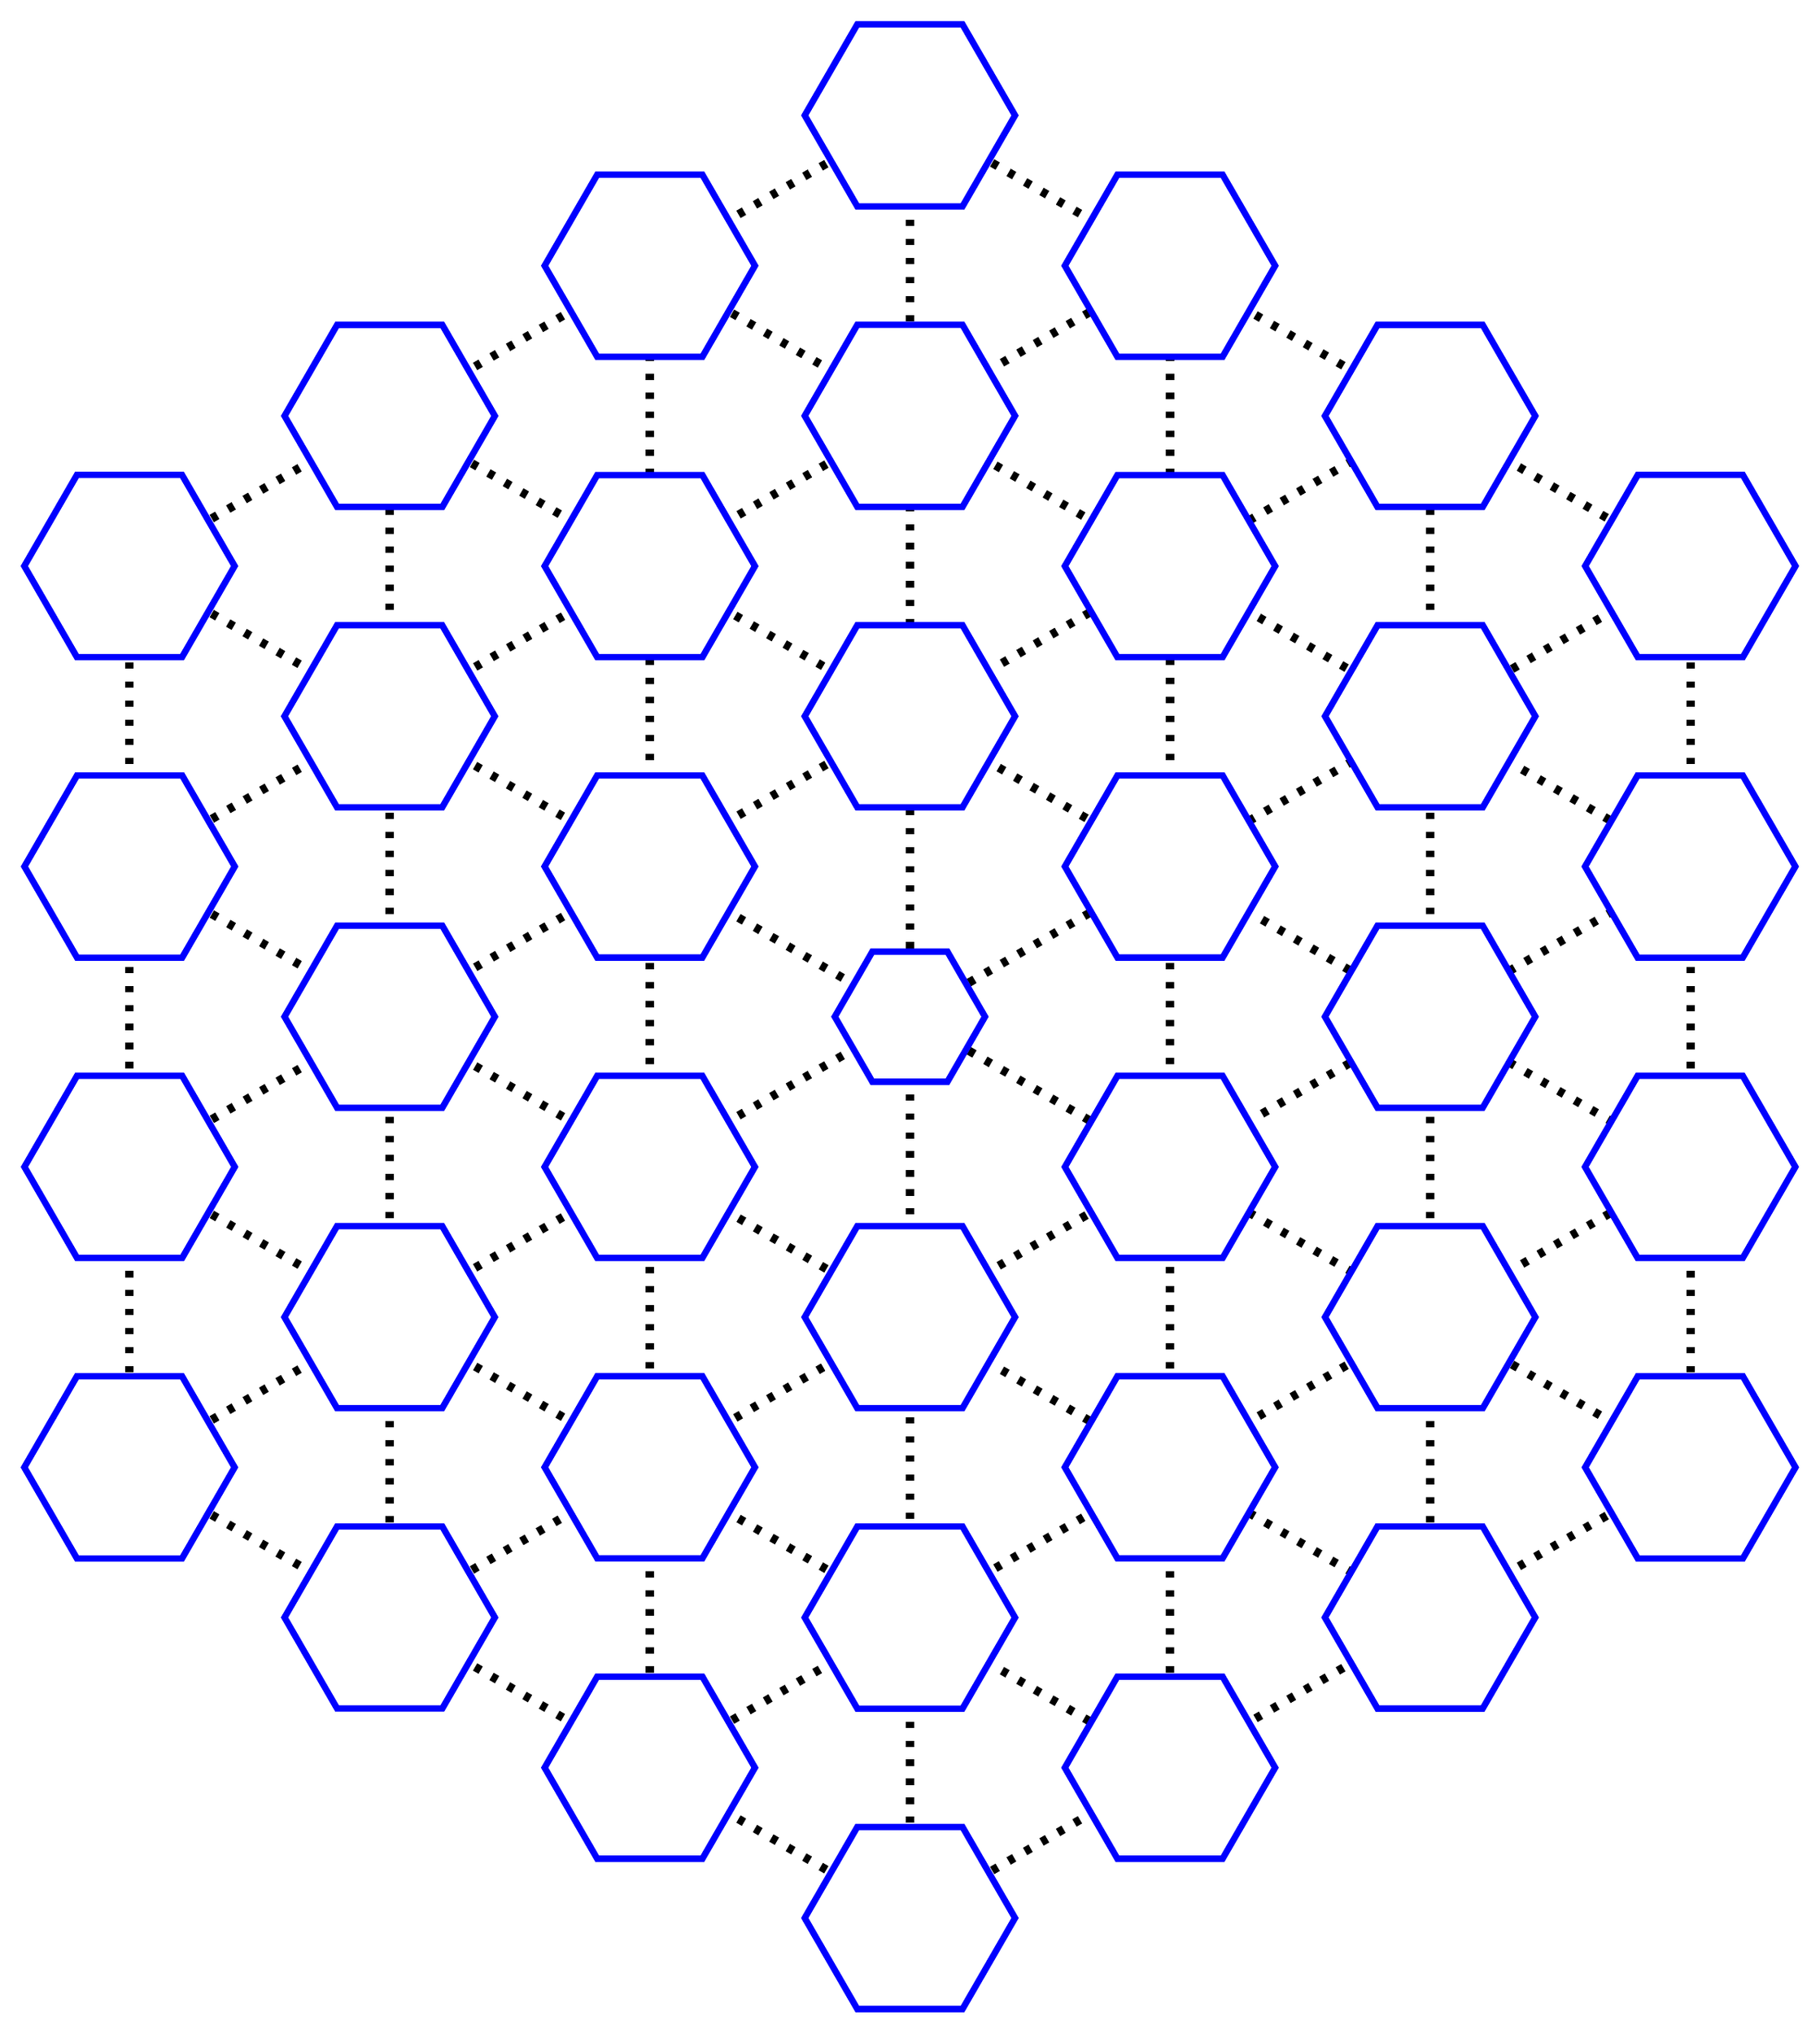
\begin{tikzpicture}[scale=5, rotate around={90:(10,0)}]
%%%  define vertices with coordinates
\coordinate (0;0) at (0,0); 
\foreach \c in {1,...,3}{%  
	\foreach \i in {0,...,5}{% 
		\pgfmathtruncatemacro\j{\c*\i}
		\coordinate (\c;\j) at (60*\i:\c);  
} }
\foreach \i in {0,2,...,10}{% 
	\pgfmathtruncatemacro\j{mod(\i+2,12)} 
	\pgfmathtruncatemacro\k{\i+1}
	\coordinate (2;\k) at ($(2;\i)!.5!(2;\j)$) ;}

\foreach \i in {0,3,...,15}{% 
	\pgfmathtruncatemacro\j{mod(\i+3,18)} 
	\pgfmathtruncatemacro\k{\i+1} 
	\pgfmathtruncatemacro\l{\i+2}
	\coordinate (3;\k) at ($(3;\i)!1/3!(3;\j)$)  ;
	\coordinate (3;\l) at ($(3;\i)!2/3!(3;\j)$)  ;
}

%%%%%%%%% draw lines %%%%%%%%
\foreach \i in {0,...,6}{% 
	\pgfmathtruncatemacro\k{\i}
	\pgfmathtruncatemacro\l{15-\i}
	\draw[line width=4pt,black,loosely dashed] (3;\k)--(3;\l);
	\pgfmathtruncatemacro\k{9-\i} 
	\pgfmathtruncatemacro\l{mod(12+\i,18)}   
	\draw[line width=4pt,black,loosely dashed] (3;\k)--(3;\l); 
	\pgfmathtruncatemacro\k{12-\i} 
	\pgfmathtruncatemacro\l{mod(15+\i,18)}   
	\draw[line width=4pt,black,loosely dashed] (3;\k)--(3;\l);}    
%%%%%%%%% draw points %%%%%%%% 
\node[regular polygon, regular polygon sides=6,draw,
minimum width=2.5cm,
outer sep=0,line width=3pt,blue,fill=white] at (0;0) {};
\foreach \c in {1,...,3}{%
	\pgfmathtruncatemacro\k{\c*6-1}    
	\foreach \i in {0,...,\k}{% 
	\node[regular polygon, regular polygon sides=6,draw,
	minimum width=3.5cm	,outer sep=0,line width=3pt,blue,fill=white] at (\c;\i) {};
}}  


 
 
 
\end{tikzpicture}



\end{document}	
	